\documentclass[a4paper,12pt]{article}



% Pacotes essenciais
\usepackage[brazil]{babel}
\usepackage[T1]{fontenc}

% Pacotes para citações no estilo ABNT
\usepackage[alf]{abntex2cite}

% Pacotes adicionais
\usepackage{csquotes, graphicx, xcolor, comment, enumerate, multirow, 
    multicol, titlesec, amsmath, amsthm, amsfonts, amssymb, dsfont, 
    blindtext, ragged2e, array, enumitem, tikz, bbding, pifont, wasysym, 
    titling, longtable, fancyhdr, url, float, placeins, xurl}

\usepackage{graphicx}\usepackage[table]{xcolor}
% Configuração de margens
\usepackage[lmargin=2cm, rmargin=2cm, tmargin=2cm, bmargin=2.5cm]{geometry}

% Configuração do cabeçalho com logo
\usepackage{fancyhdr}
\pagestyle{fancy}
\fancyhf{}
\renewcommand{\headrulewidth}{0pt} % Remove a linha no cabeçalho
\rhead{\transparent
\includegraphics[width=2cm]{./assets/logocogel.jpg}} % Certifique-se do caminho correto

% Configuração do hyperref (deve ser o último pacote)
\usepackage{hyperref}
\hypersetup{
    colorlinks=true,
    linkcolor=blue, % Cor dos links internos (tabelas, figuras, etc)
    urlcolor=blue,  % Cor dos links externos
    citecolor=green % Cor das citações
}

\usepackage{helvet}
\renewcommand{\familydefault}{\sfdefault}

% Configuração da bibliografia (ABNT)
\bibliographystyle{abntex2-alf}
 
\title{Relatório de Auditoria de Segurança Cibernética}
\author{}
\date{}
\begin{document}


\begin{center}
    \large{\textbf{Companhia de Governança Eletrônica do Salvador\\
Diretoria Técnica e de Infraestrutura\\
Gerência Especial de Segurança da Informação\\
}}

\vspace{7cm}

\Large{Relatório de Auditoria de Segurança Cibernética\\
[NOME SECRETARIA] - [SIGLA]}

\vspace{4cm}
\textcolor{red}{CONFIDENCIAL}
\end{center}
\newpage

\tableofcontents  %Sumario


\newpage

\section{Introdução}
\subsection{Objetivo}
Este relatório, elaborado pela \textbf{Gerência Especial de Segurança da Informação da COGEL}, apresenta os resultados da auditoria de segurança cibernética realizada no ambiente de aplicações e servidores da Prefeitura de Salvador, administrado pela empresa [NOME SECRETARIA] - [SIGLA]. O objetivo principal é identificar vulnerabilidades e riscos associados à segurança da informação, avaliar a conformidade com as normas e padrões de segurança aplicáveis, e fornecer uma visão abrangente do estado atual da segurança cibernética no ambiente auditado.

\subsection{Escopo}
A auditoria abrange a avaliação das vulnerabilidades em sistemas operacionais e aplicações web, identificadas no período de [INICIO DATA] a [FIM DATA].

\section{Metodologia}
\subsection{Ferramentas Utilizadas}
\begin{itemize}
    \item \textbf{Tenable.io Vulnerability Management (Nessus, NNM):} Esta ferramenta avançada de gerenciamento de vulnerabilidades permite a realização de escaneamentos automatizados para identificar falhas de segurança em sistemas e redes. Utiliza diversas técnicas de varredura para detectar vulnerabilidades conhecidas e potenciais, ajudando a priorizar a correção com base em riscos específicos.
    \item \textbf{Trend Micro XDR Vision One:} Plataforma de Detecção e Resposta Estendida (XDR) que oferece visibilidade abrangente e correlação de ameaças em múltiplos vetores, incluindo endpoints, servidores e redes. A ferramenta melhora significativamente a capacidade de resposta a incidentes, correlacionando dados de diferentes fontes para identificar atividades maliciosas de forma mais eficaz.
    \item \textbf{Microsoft Windows:} Sistema operacional desenvolvido pela Microsoft, amplamente utilizado em ambientes corporativos e pessoais. Conhecido por sua interface amigável e vasta gama de aplicações empresariais, o Windows também incorpora diversas ferramentas de segurança e gerenciamento, como o Windows Defender e o Active Directory.
    \item \textbf{Linux:} Sistema operacional de código aberto amplamente utilizado em servidores e desktops. Reconhecido por sua robustez, segurança e flexibilidade, o Linux suporta uma vasta gama de distribuições que podem ser otimizadas para diferentes propósitos, desde servidores de alta performance até dispositivos embarcados.
\end{itemize}

\subsection{Procedimentos}
A auditoria foi conduzida por meio de uma série de escaneamentos automatizados, inspeções manuais e validações de conformidade com as normas e padrões de segurança aplicáveis.

\section{Sumário Executivo}
A auditoria revelou um total de \textbf{[TOTAL VULNERABILIDADES]} ativas, distribuídas entre críticas, altas, médias e baixas. A seguir, apresentamos um resumo das principais descobertas.

\section{Análise de Vulnerabilidades e Riscos Associados}
As vulnerabilidades identificadas apresentam um risco significativo para a segurança do ambiente de TI da Prefeitura de Salvador. A seguir, destacamos os principais riscos associados a essas vulnerabilidades:

O escaneamento de vulnerabilidades dos hosts levantou um total de \textbf{[TOTAL VULNERABILIDADES VM]} vulnerabilidades, classificadas em críticas, altas, médias e baixas.

   \begin{figure}[h!]
    \centering
    \includegraphics[width=0.4\textwidth]{assets/images-vmscan/Total_Vulnerabilidades.png} 
    \end{figure}
    \FloatBarrier

A seguir, destacamos os principais riscos associados a essas vulnerabilidades: 

[RELATORIO SERVIDORES]

%-------------------------------------------------------------------------------------------------
\section{Riscos Associados à Segurança de Aplicações}

Esta seção tem como objetivo apresentar e detalhar as vulnerabilidades relacionadas às aplicações web, destacando a quantidade de ocorrências em cada um dos \textbf{[TOTAL_SITES]} sites pertencentes a [NOME SECRETARIA] - [SIGLA]. Além disso, são fornecidas descrições detalhadas e recomendações de mitigação para cada tipo de vulnerabilidade identificada.\\

Os escaneamentos de vulnerabilidades foram realizados com a ferramenta \textit{Tenable}, e os relatórios completos estão disponíveis para consulta no seguinte link: \url{[GOOGLE DRIVE LINK]}.\\

O levantamento \textbf{total resultou em [TOTAL VULNERABILIDADES WEB] vulnerabilidades}, distribuídas em diferentes níveis de severidade. Essas vulnerabilidades foram classificadas da seguinte forma: [TOTAL VULNERABILIDADES WAS CRITICA] como crítica(\textit{Critical}), [TOTAL VULNERABILIDADES WAS ALTA] como altas (\textit{High}), [TOTAL VULNERABILIDADES WAS MEDIA] como médias (\textit{Medium}) e [TOTAL VULNERABILIDADES WAS BAIXA] como baixas (\textit{Low}). A distribuição dessas vulnerabilidades é ilustrada no gráfico a seguir, que facilita a compreensão do impacto potencial na segurança das aplicações.

\begin{figure}[h!]
    \centering
    \includegraphics[width=0.5\textwidth]{assets/images-was/Total_Vulnerabilidades.png}
    \caption{Distribuição total de vulnerabilidades por severidade}
\end{figure}
\FloatBarrier

Abaixo, encontra-se um gráfico que apresenta o total de vulnerabilidades por site. Para um detalhamento mais específico sobre os quantitativos de vulnerabilidades de cada site, recomenda-se acessar os relatórios individuais de cada aplicação.

\begin{figure}[h!]
    \centering
    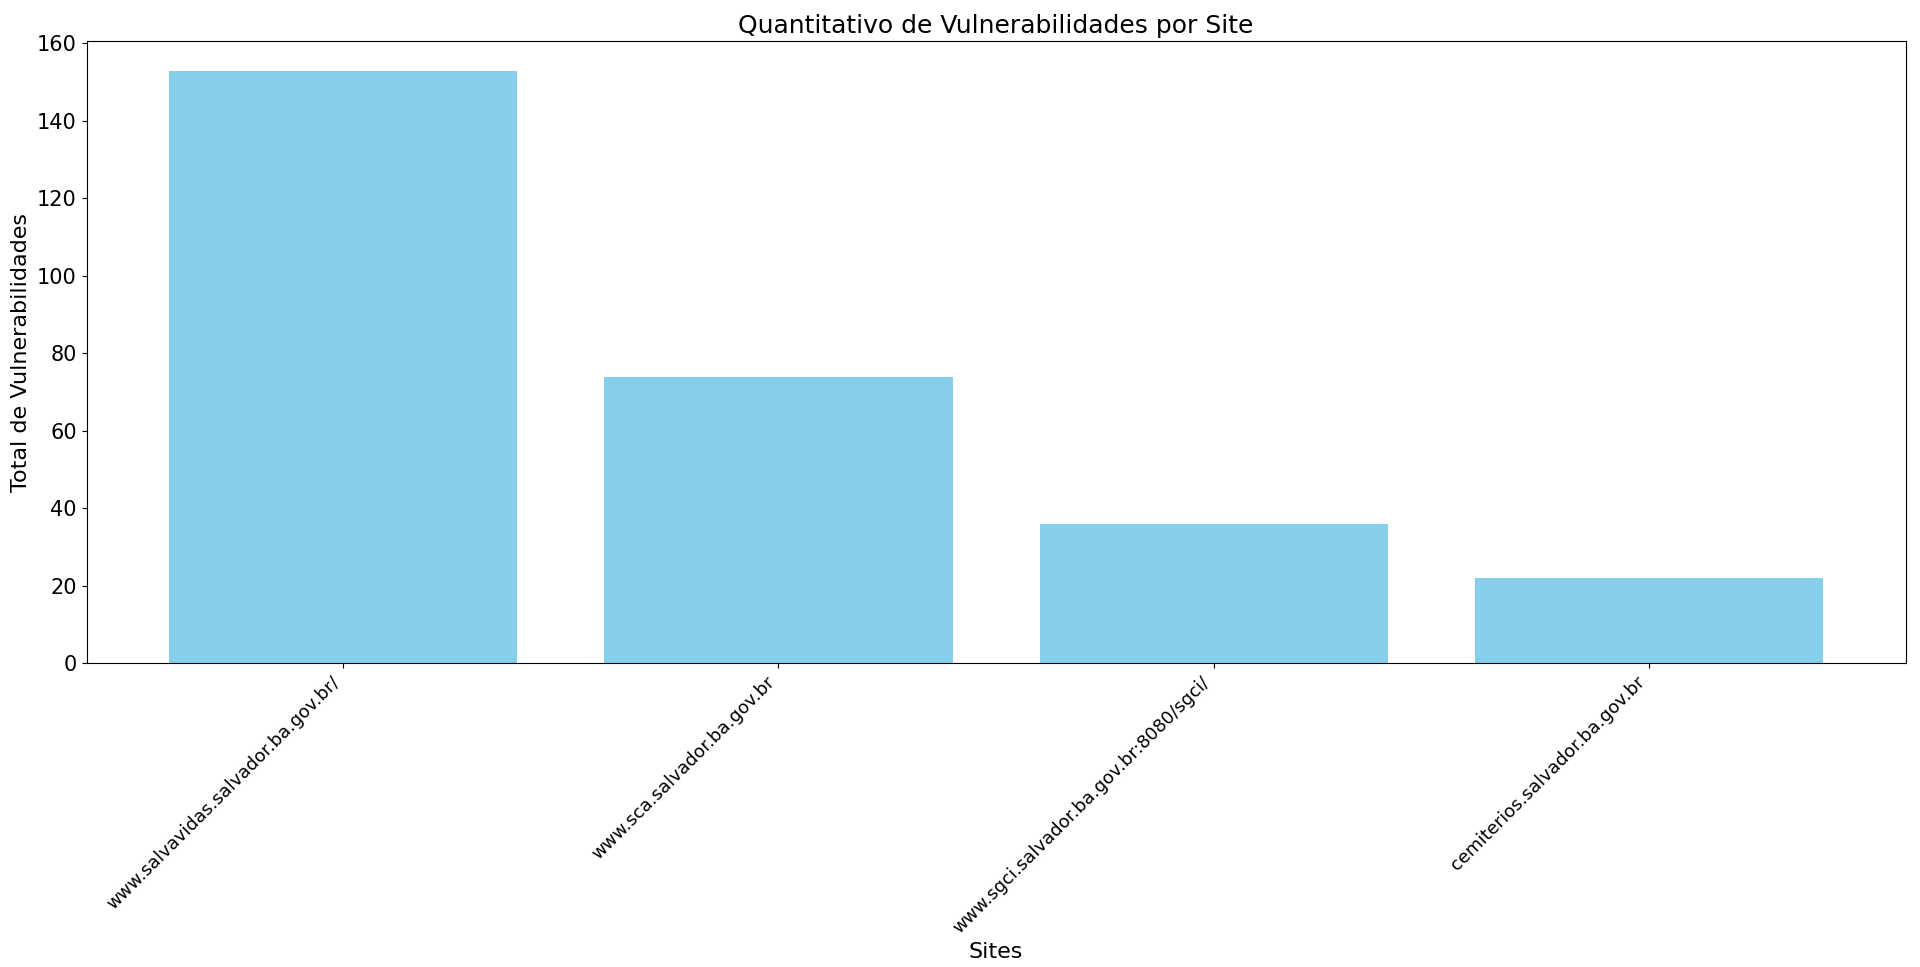
\includegraphics[width=1.0\textwidth]{assets/images-was/Vulnerabilidades_x_site.png}
    \caption{Total de vulnerabilidades por site}
\end{figure}
\FloatBarrier
As vulnerabilidades identificadas foram organizadas em seções e subseções, com o intuito de agrupá-las de acordo com sua afinidade e severidade. Cada seção aborda um conjunto específico de falhas de segurança, desde as relacionadas à configuração de segurança dos protocolos HTTP e TLS, até questões relacionadas à configuração inadequada do servidor e à exposição desnecessária de informações sensíveis. As subseções detalham vulnerabilidades em áreas como segurança de cookies e sessões, injeções de código, falhas de autenticação, entre outras. Essa estrutura facilita a análise, permitindo uma compreensão clara dos riscos e das recomendações de mitigação associadas a cada tipo de vulnerabilidade identificada.

%-------------- INÍCIO DA CATEGORIA Vulnerabilidades Relacionadas a Configurações de Segurança HTTP E TLS --------------
[RELATORIO GERADO]
%-------------- FIM DA CATEGORIA Outras Vulnerabilidades Críticas e Explorações --------------
\section{Conclusão}

A auditoria de segurança cibernética realizada pela Gerência Especial de Segurança da Informação da COGEL revelou um cenário alarmante de vulnerabilidades e riscos no ambiente de aplicações e servidores da Prefeitura de Salvador, administrado pela  [NOME SECRETARIA] - [SIGLA]. Foram identificadas diversas vulnerabilidades ativas, incluindo falhas críticas, altas, médias e baixas, que expõem o ambiente a possíveis ataques cibernéticos. Problemas graves, permissões incorretas de aplicações, suporte a protocolos e cifras criptográficas inseguras, e configurações inseguras em Sistemas Operacionais para aplicações críticas e a utilização de sistemas não suportados foram destacados.\\

A presença dessas vulnerabilidades representa uma ameaça significativa à segurança da informação e à continuidade dos serviços da Prefeitura de Salvador. A adoção de políticas de segurança mais rigorosas e a conformidade com normas como ISO/IEC 27001, NIST SP 800-53 e PCI DSS são essenciais para fortalecer a postura de segurança cibernética da instituição. A urgência na aplicação de patches e na implementação de medidas corretivas é imperativa para mitigar esses riscos e proteger a integridade, confidencialidade e disponibilidade dos serviços e dados da prefeitura e de seus cidadãos.\\

Por atingir seu objetivo, esta comissão encerra o presente instrumento ao tempo que declara o fim da Auditoria de Segurança Cibernética do Ambiente da [NOME SECRETARIA] - [SIGLA].

\newpage

\vspace*{\fill} % empurra o conteúdo para o final da página
\begin{flushright}
\textbf{Salvador, [MES CONCLUSAO] de [ANO CONCLUSAO] \\%
Gerência Especial de Segurança da Informação \\%
Diretoria Técnica e de Infraestrutura \\%
Companhia de Governança Eletrônica do Salvador}
\end{flushright}

\end{document}
